%\chapter{Spatial Capture-Recapture for Unmarked Populations}
\chapter{Unmarked Populations}
\markboth{Unmarked Populations}{}
\label{chapt.scr-unmarked}

\vspace{0.3cm}

Traditional capture-recapture models share the fundamental
assumption that each individual in a population can be uniquely
identified when captured. Often, this can be accomplished
by marking individuals with color bands, ear tags, or some other
artificial mark that subsequently can be read in the field. For other
species, such as tigers (\textit{Panthera tigris}) or
marbled salamanders (\textit{Ambystoma opacum}),
individuals can be identified
using only their natural markings. However, many species
do not possess adequate natural markings and are
difficult to capture, making it impractical to use standard
capture-recapture techniques.

Estimating density when individuals are unmarked can be accomplished
using a variety of alternatives to capture-recapture, such as distance
sampling \citep{buckland_etal:2001} and $N$-mixture models
\citep{royle:2004biom}.
% XX RS: Here would be a good point to mention the gas model, since it's another option for density estimation. You might also want to say something about the use of indices, since it's what people often do when they can't formally estimate abundance (and even sometimes when they can). I don't think these things are essential here, but might fit well.
% XX RS later: Ok, I see this stuff comes up below.
These methods, among others, can be
very effective when their assumptions are met, but in cases such as
when it is not possible to obtain accurate distance data, or when
movement complicates the use of fixed-area plots,
these methods may not yield unbiased estimates of density
\citep{chandler_etal:2011}.
% XX RS: I'd also add that direct observation based methods cannot
% usually be applied to cryptic species.
% RC: Done.
Furthermore, some species are so rare and
cryptic that it is nearly impossible to collect enough data using
traditional survey methods.

In this chapter, we investigate spatially explicit alternatives for estimating density
of unmarked populations, and we highlight the work of
\citet{chandler_royle:2012} who demonstrated that the ``individual
recognition'' assumption of traditional capture-recapture models is not a
requirement of spatial capture-recapture models. They showed that,
under certain conditions, % described below,
spatially correlated count
data are sufficient for making inference about animal distribution and
density even when no individuals are marked.
The \citet{chandler_royle:2012} ``spatial count model'' (hereafter the SC
model) requires neither distance data nor fixed area plots. Instead,
the observed data are trap- and occasion-specific counts, which
are modeled as a reduced-information summary of the \textit{latent}
encounter histories. Because the model is formulated in terms of the
data we wish we had, i.e. the typical encounter history data observed
in standard capture-recapture studies of marked animals, the SC model
is just a SCR model with a single extension to account for the fact
that the encounter history data are unobserved. However, this results
in a drastically different model than the models typically used for
count data in ecology because the SC model is parameterized in terms of
individuals, and specifically, their locations relative to the
sampling device.

The ability to fit SCR models to data from unmarked populations has
important implications. For one, it means that SCR models can
be applied to data collected using methods like points counts in which
observers record simple counts of animals at an array of survey
locations. The model can also be fitted to camera trapping data collected on
unmarked animals, representing one of the first formal method for estimating
% XXXX Mention gas model?
% XX RS: Yeah, I think you should acknowledge the gas model, since it existed before.
%and prior to the SC models
%there were few, if any, options for modeling
% XXX RC: Ok, brief mention here, and I now discuss it in more depth below
density from such data \citep[but see][]{rowcliffe_etal:2008}.
So, is the SC model a free lunch? At face value, it sounds as though it
allows for estimation of
%can estimate
all the quantities of interest in standard
capture-recapture studies, but with very little
data. But of course the answer is no --
%The answer is of course not---
lunch is still not free because
with this model come new assumptions,
%which we will describe in this chapter,
and as was demonstrated by
\citet{chandler_royle:2012}, even with ``perfect'' data, parameter estimates
will typically not be very precise. This should not be surprising
given that we are asking so much from simple count data.

The real value of the SC model is two-fold. First, it demonstrates
an important theoretical result, namely
that spatial correlation in
count data carries information about density and distribution -- and this
% XX RS: and density?
% XX RC: done
%of individuals.
stands in stark contrast to a prevailing view of
spatial correlation as a nuisance to be avoided or modeled out of unsightly
residual plots. The second reason why this model is important is that
it provides the basis for numerous model extensions that \textit{can}
result in precise estimates of density. % when some or all of the
%individuals in a population are unmarked.
We will discuss some of
these possibilities in this chapter, but
% handling the extremely common phenomenon in
%which only a subset of individuals in a population can be marked or otherwise
%distinguishable.
%Thus, while we do not recommend foregoing the work
%required to mark animals, this model does provide a method for
%studying unmarked populations, which \textit{can} yield precise
%density estimates if some of the individuals are marked, or if prior
%information about some of the parameters is available.
perhaps the most useful extension -- accomodating %of this model
data from marked and unmarked
individuals -- is treated separately in the next chapter. Here, we focus
on situations in which all individuals are unmarked, and
we begin by presenting the most basic formulation of the model. Then we proceed, by
way of a few examples, to consider extensions of the model in which
ancillary information can be used to increase precision.

\section{Existing Models for Inference About Density in Unmarked Populations}
\label{Sect.existing-unmarked}
% XX RS: I think in this section it would be good to cite the Williams
% et al 2002 book - they have a really nice chapter on indices and the
% book is such a standard volume.
% XX RC: done
When capture-recapture methods are not a viable option, ecologists
often collect simple count data or even binary detection/non-detection
data. %to estimate parameters such abundance or occupancy.
%\citep{royle:2004biom, mackenzie_etal:2002}.
These data are often treated as an index of abundance or occurrence
and are analyzed using generalized linear models such as
Poisson regression or logistic regression, perhaps with random
effects \citep{zuur_etal:2009}. %When detection is imperfect, as it almost always is,
However, index methods cannot be used to make unbiased inferences
about abundance or occurrence unless strong assumptions about constant
detection probability are valid
\citep{williams_etal:2002,sollmann_etal:2013bioc}.
%when detection is imperfect, as
%it usually is. Even when count data or detection/non-detection data are
%used as an index of abundance or occurrence,
In particular,
index methods can be highly misleading
%unreliable results
when covariates affect both the ecological process of interest
and the observation process. A classic example is given by
\citet{bibby_buckland:1987} who found that songbird detection
probability was negatively related to vegetation height, whereas
density was positively associated with vegetation height in restocked
conifer plantations. This intuitive phenomenon has been
demonstrated repeatedly \citep[e.g.][]{kery:2008,sillett_etal:2012} and has led to the
development of a vast number of models to estimate population size and
occurrence probability when individuals are unmarked and detected
imperfectly
\citep{buckland_etal:2001,williams_etal:2002,mackenzie_etal:2006,royle_dorazio:2008}.
A review of these
models is beyond the scope of this
chapter, but we mention a few deficiencies of existing methods
that warrant the exploration of alternatives for robust inference when
standard capture-recapture methods do not apply.

Distance sampling \citep{buckland_etal:2001,buckland_etal:2004book}, which we briefly
introduced in Chapter~\ref{chapt.closed},
is perhaps the most widely used method for
estimating population density when individuals are unmarked and
detection probability is less than one. This class of methods is known
to work impeccably when estimating the number of stakes in a field or
the number of duck nests in a wetland. Distance sampling can also work very well in
more interesting situations, and it is an extremely powerful method when
the assumptions can be met. However, the assumptions that distance
data can be recorded without error and that animals are distributed
randomly with respect to the transect can be easily violated by
common processes such as animal movement and measurement
error. Although numerous methods have been proposed to
relax some of these assumptions
\citet{royle_etal:2004, borchers_etal:1998, johnson_etal:2010,
  marques_etal:2010, chandler_etal:2011},
a more important issue is that distance
sampling is simply not practical in many settings. For example, many
species are so rare and elusive that they can only be reliably
surveyed using ``indirect'' methods such as camera traps or hair
snares.

In response to the increasing use of camera traps in studies of
threatened species, and the problems associated with commonly-used
indices of abundance %from such data
\citep{jennelle_etal:2002,obrien:2011,sollmann_etal:2013bioc},
several density estimators
have been developed for situations in which the population being
studied is unmarked \citet{rowcliffe_etal:2008,rowcliffe_etal:2011}.
These estimators assume that (1) cameras are randomly placed with
respect to animal density (2) animals neither avoid nor are attracted
to the cameras, and (3) detection probability can be either modeled as a function of
distance between the animal and the camera or as a function of
movement velocity. Although these methods may
represent an important improvement over index-based methods,
the assumptions may not hold in many situations, especially when
applied to data from standard designs in which camera stations are
either baited or placed along trails -- issues that can be dealt with
directly using SCR models (see Chapts.~\ref{chapt.ecoldist} and~\ref{chapt.rsf}).
Nonetheless, empirical studies
have found that the assumptions do hold in some cases
\citep{rowcliffe_etal:2008}.

Other common approaches to estimating density when individuals are
unmarked include double observer sampling, removal sampling, and
repeated counts, for which custom models have been developed
\citep{nichols_etal:2000, farnsworth_etal:2002, royle:2004biom,
  royle:2004abc, nichols_etal:2009,fiske_chandler:2011}. To
obtain reliable density estimates using these
methods, the area surveyed must be well defined and closed with
respect to movement and demographic processes. Given a sufficiently short
sampling interval, such as a 5-min point-count, the closure
assumption may be reasonable. However, short sampling intervals limit
the number of detections, so observers generally visit each survey
location multiple times during a season. But then, animal
movement may invalidate the closure assumption, and a model of
temporary emigration is required
\citep{kendall_etal:1997,chandler_etal:2011}. Furthermore,
distance-related heterogeneity in detection probability can introduce
bias in these models, although this bias is negligible when the
ratio of plot size to the scale parameter of the detection function is low
\citep{efford_dawson:2009}.

We mention these issues not to suggest that existing models do not
have value -- indeed we believe that they can be used to obtain
reliable density estimates in many situations -- rather, our aim is to
highlight the need for alternative methods when the assumptions of
existing methods cannot be met and when spatially-explicit inference
is the objective. %Additionally, the spatial count model
%we discuss in this chapter serves as the foundation for a broad class
%of SCR models in which all or some of the individuals cannot be
%uniquely identified, which is the focus of the next chapter.

%% XXX RS: I copy-pasted a little paragraph on the gas model below, in
%% case you want to use that to mention this model here. I think,
%% since you discuss these alternatives, it would be nice to
%% acknowldge the existence this model as well.

% Another option is the trap encounter rate model by Rowcliffe
% et al. (2008), which estimates density as a function of encounter
% rates between animals and traps, animal movement speed and
% rate. The model assumes random
% movement of individuals and requires a completely random trap
% setup relative to animal movement, which can result in prohibitively low numbers of photographs,
% and may logistically not be feasible at all. It further
% requires knowledge of, or the ability to estimate, movement speed
% and the amount of time individuals are active.

\section{Spatial Correlation in Count Data}

\subsection{Spatial correlation as information}
\label{sect.corr-info}

All of the previous methods require some sort of auxiliary information
to model both abundance and detection. For instance, %we might need
multiple observers, distance data, or repeated visits
may be required to ensure
that model parameters are identifiable
\citep[but see][]{lele_etal:2012, solymos_etal:2012}. The same is true for
the SC model, but the auxiliary information comes in the form of spatial
correlation, which requires no extra effort to collect
\citep{chandler_royle:2012}. %In fact, it's probably safe to say that
%it is harder to avoid spatial correlation that it is to

It is natural to be suspicious of the claim that spatial correlation
is a good thing. In fact, elaborate methods have been devised to deal
with spatial correlation as a nuisance %parameter
\citep{lichstein_etal:2002,dormann_etal:2007}, and ecologists have been admonished for
failing to obtain ``real'' replicates uncontaminated by spatial
correlation \citep{hurlbert:1984}. The following heuristic may be
helpful for seeing the value of spatial correlation
in the context of density estimation.
% XX RS: maybe add 'in the context of density estimation'

Imagine a $10 \times 10$ grid of camera traps and a single unmarked
individual exposed to ``capture'' whose home range center lies in the center of the
trapping grid. If the individual has a small home range size relative
to the extent of the trapping grid, we can envision what the
spatial correlation structure of the encounters might look
like. If the animal's home range is symmetric around the activity center
then the number of times the individual is detected at each
trap (the trap count) should decrease with the distance between the home
range center and the trap; i.e., traps with the same distance
from the activity center will yield counts that are more highly
correlated with one another than traps located at different distances
from the activity center. Thus, the correlation among the counts tells us
something about the location of the activity center. It is relatively
intuitive that spatial correlation carries information about
distribution, but what about density?


Imagine now that there are two activity centers located in the trapping
grid. Using trap counts alone, %which allow for imperfect detection,
is it possible to determine the number and location of these activity
centers? The answer is yes, at least under certain circumstances.
Fig.~\ref{chapt-unmarked.fig.heur}
shows the locations of the two hypothetical activity centers, and the total
counts obtained at each trap after 10 survey occasions.
%distance between the sampling location and the individual.
Assuming that animals have bivariate normal home
ranges, the fact that there are two areas in the map with high counts
that dissipate with distance suggests that the most likely number of
individuals given these data is 2. Furthermore, the degree to which
the counts dissipate from the two areas of highest intensity is
information about the parameter governing home range size. These two
pieces of information are enough to estimate the number of
individuals exposed to sampling -- again, given
that a bivariate normal home range is a valid assumption. Of course,
the data could just as well have been generated by a single individual
whose home range is distinctly bimodal, and thus \textit{as always}
the assumptions of our model need to be carefully examined using our
biological knowledge of the system. If the assumptions
do not hold, it is almost always possible to relax them, for instance
by allowing for non-stationary home ranges as we demonstrated in
Chapt.~\ref{chapt.ecoldist} and~\ref{chapt.rsf}.

\begin{figure}%[ht!]
\centering
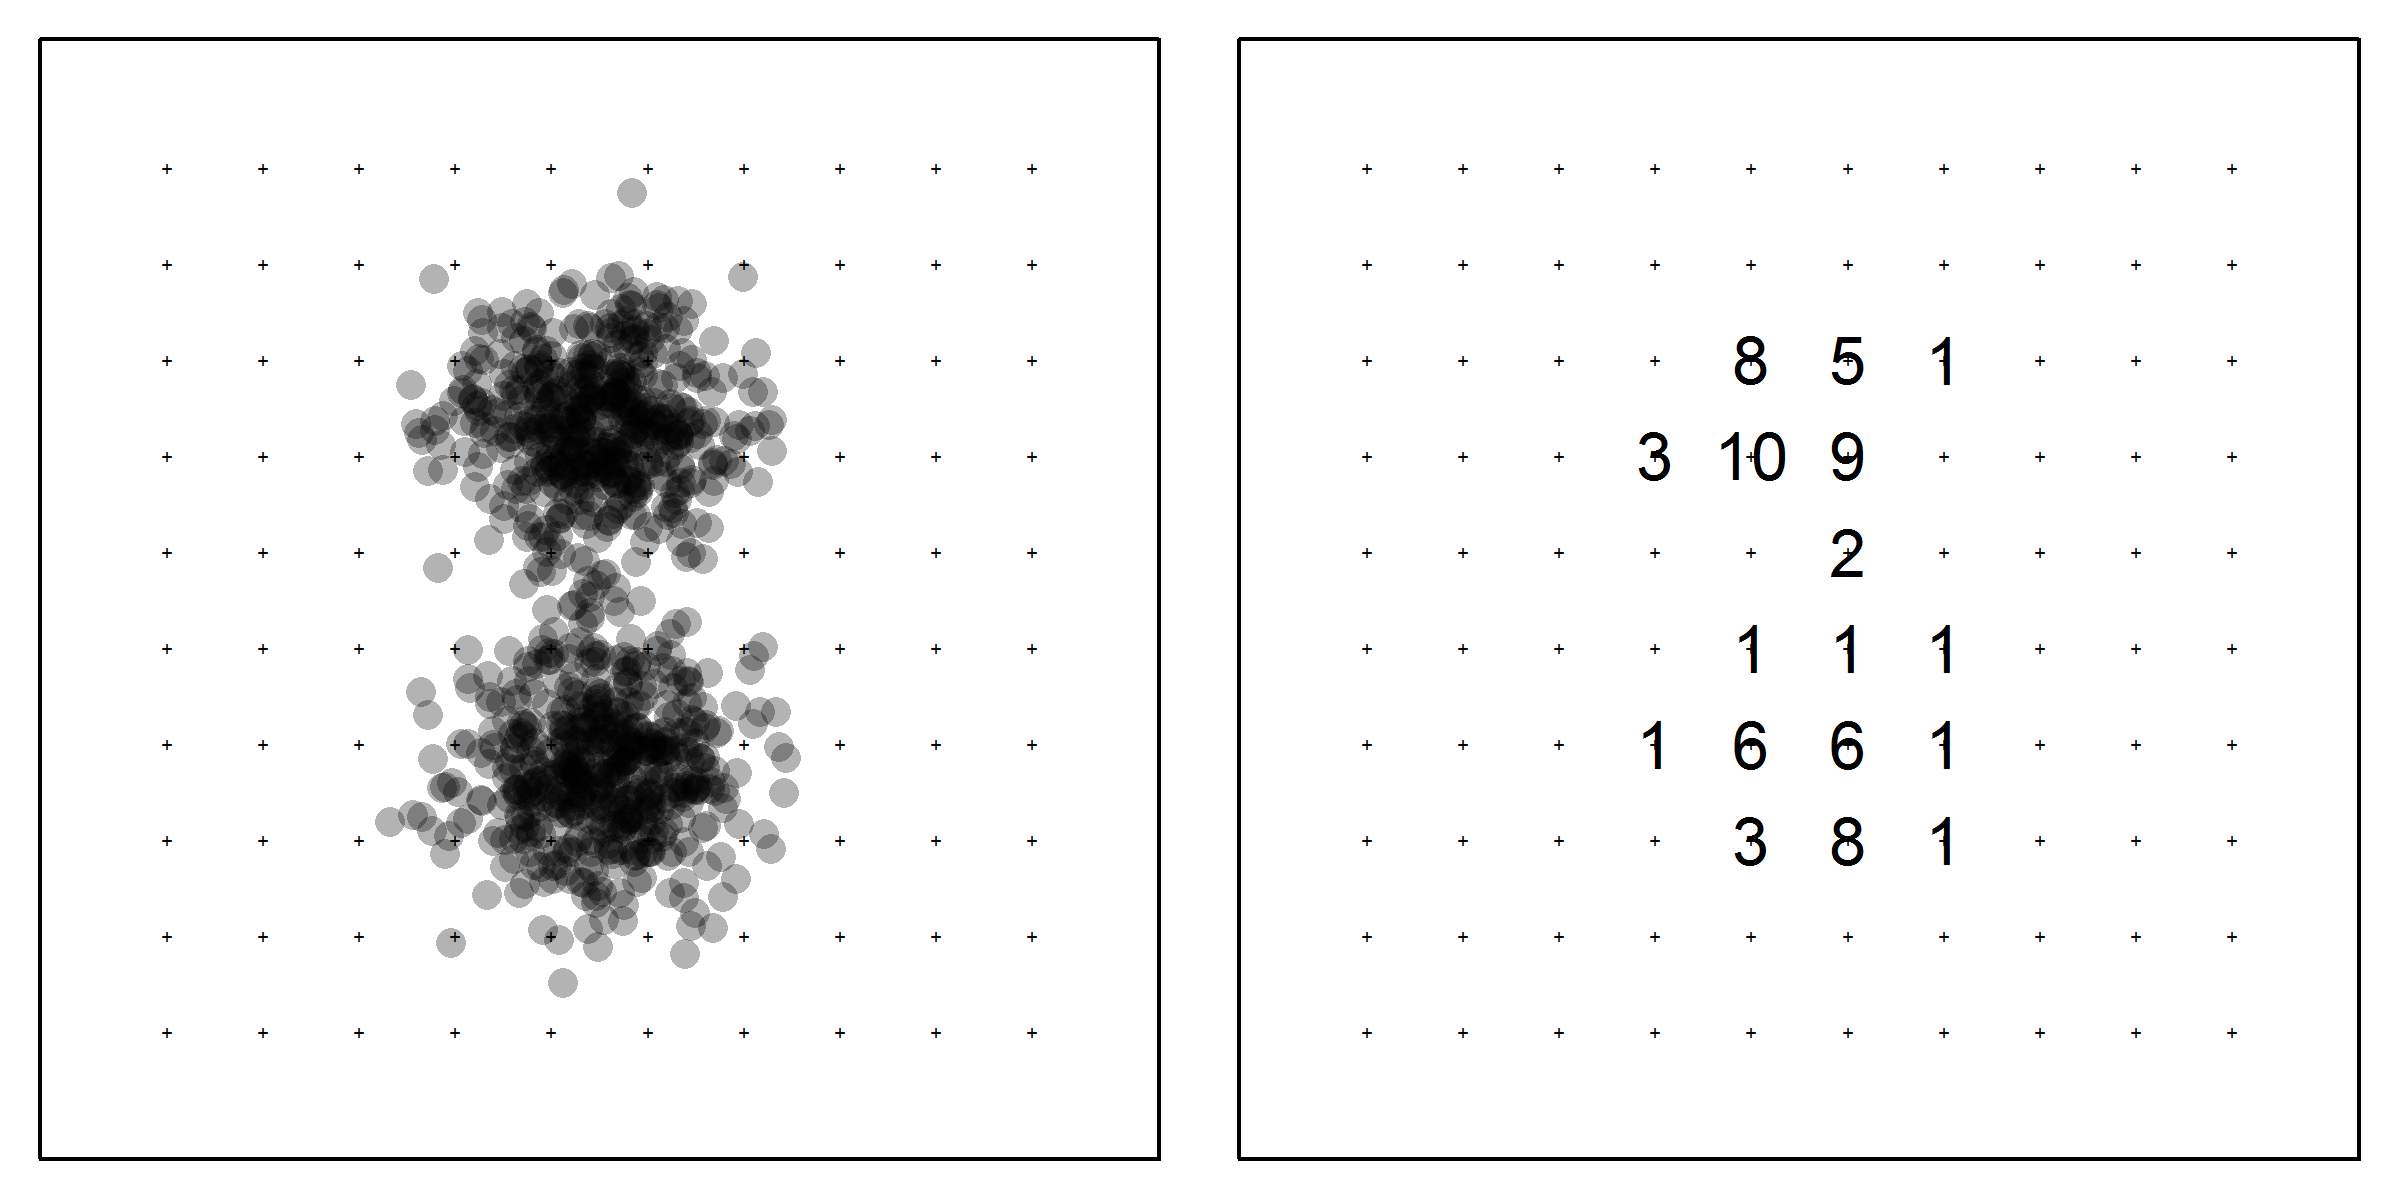
\includegraphics[width=0.5\textwidth]{Ch18-Unmarked/figs/heuristic}
\caption{Simulated count data at each of 100 camera traps
  (crosses) after $K=10$ sampling occasions. The black dots are the
  locations of two animal activity centers. The
  spatial count model estimates %attempts to estimate
  both the location and number of activity centers exposed to
  sampling using such spatially-referenced count data.}
\label{chapt-unmarked.fig.heur}
\end{figure}




\subsection{Two types of spatial correlation}

The spatial correlation dealt with by the SC model is assumed to arise
from animal movement; however, this is just one type of spatial
correlation that may exist in ecological count data. Another common
type of spatial correlation results from the spatial correlation of
environmental covariates. Habitat variables, such as, for example, the percent cover
of deciduous forest in North America, will often be patchy rather than randomly
distributed, and this can result in spatial correlation in abundance,
and hence in count data.  %as
Often, this type of spatial correlation can be dealt with by simply including
the habitat covariate in the model. For example, a simple, non-spatially-explicit
species distribution model with only a few habitat variables can result in a
distribution map that reflects the spatial correlation in abundance
\citep{sillett_etal:2012,royle_etal:2012mee2}. %In such a case, there is no
%need to use spatially-explicit models %such as
%conditionally-autoregressive models or similar
%\citep{besag_kooperber:1995,lichstein_etal:2002,wikle:2010}.
The point is that the %reason is that the
relevant assumption of non-spatial models (e.g. GLMs) is that
no spatial correlation exists in the \textit{residuals}, and often,
any spatial correlation apparent in the counts can be accounted for using
covariates. This may be obvious, but
it is a point that seems to be frequently misunderstood.

Of course, sometimes spatial correlation exists in residuals even
after including covariate effects. %It does become
%important to account for environmentally-induced spatial correlation
%in situations where correlation exists in the residuals
%\textit{after} accounting for covariate effects.
This may be due to
%movement, as we discuss in this chapter, or it may be due to
unobserved covariates or unobserved processes such as dispersal. When
mechanistic models cannot be developed to describe these processes,
several options exist for handling spatial correlation as a nuisance
parameter \citep{besag_kooperber:1995,zuur_etal:2009,wikle:2010}. % offer advice on
%how to check for and deal with such correlation in the context of
%spatial correlation in the residuals of
%GLMs and GLMMs. %In the case of SCR models, such correlation
In the context of SCR models, including the SC model dealt with in this
chapter, movement-induced spatial correlation is always explicitly
modeled, and other sources of spatial correlation can be accounted for
as well. For instance,
%account for movement-induced spatial
%correlation, and they can also be used to account for
environmentally-induced spatial correlation can be modeled by adopting an
inhomogeneous point process model for the activity centers. That is,
the point process intensity can be modeled as a function of observed
covariates, and theoretically, it should be possible to allow for
spatially-correlated random effects to deal with unobserved covariates.
See Chapt.~\ref{chapt.state-space} for details.
% XX RS: Do you do that at all in the context of SC?
%Where accounting for




\section{Spatial Count Model}

\subsection{Data}

Whereas traditional SCR models require spatially-referenced
individual encounter histories, the SC model requires simple
spatially-reference count data.
Let $n_{jk}$ be the count data at sampling location $j$
on occasion $k$. The entire $J \times K$ matrix of
counts will be denoted $\bf{n}$. A sampling location in this context
could be any device capable of recording count data, such as a
human observer or a camera trap, and
one of the benefits of the SC model is that it
can be applied to data collected using many different survey
methods. For ease of presentation, we will refer to sampling devices
as traps, but remember that a trap is just something capable of
recording count data. As in all SCR models, we also require the
coordinates of the $J$ traps, and we denote the location of trap $j$
by ${\bf x}_j$. In some instances, additional data might be available such as
trap-specific covariates, state-space covariates,
information on the identities of a subset of individuals, or perhaps
even distance data. We consider some of these model extensions in
Sec.~\ref{unmarked.sec.ext}, but for the time being we ignore these %extraneous
possibilities so that we can focus on the basic model.

%The duration of sampling
%is assumed to be short enough such that the number of individuals
%exposed to sampling does not change over time.

\subsection{Model}

The state model is exactly the same as the one we have dealt with
throughout
this book. It is a point process describing the number and distribution of
activity centers in the state-space $\mathcal{S}$. Although it might
be possible to fit inhomogeneous point process models using the
methods described in Chapt.~\ref{chapt.state-space},
%we suspect thatpower to detect effects
given the simplicity of the data, we concentrate on a homogeneous point process
$\{{\bf s}_i, \ldots, {\bf s}_N\} \sim \text{Uniform}(\mathcal{S})$
where ${\bf s}_i$ is the activity center of individual $i$ in the
population of size $N$. For the moment, we will assume that $N$ is
known.

The observation model is the same as in other SCR models %covered
in the sense that it describes the probability of encountering individual
$i$ at trap $j$, conditional on the location of the individual's
activity center. The specific encounter process will depend on the
sampling method, and here we consider the standard camera trapping
situation in which an individual can be encountered at multiple traps
during a single occasion, say one night during a camera-trapping
study, and it can be detected multiple times at a single trap during
an occasion. This is the Poisson encounter model (a.k.a. the count
detector case)
%%% ANDY: I agree with Rahel here -- I changed it to count
% XX RS: If you're referring to secr I think it's the count detector.
described in Chapt.~\ref{chapt.poisson-mn}. Our
experience with alternative observation models such as the
Bernoulli and multinomial models
%that is appropriate for hair snare data
suggests that the parameters of the model may not be identifiable in
these cases, % of the Bernoulli or binomial observation models,
at least when no additional information is available. This is a subject of
ongoing research.

As before, we define $y_{ijk}$ as the
encounter data for individual $i$ at trap $j$ on occasion $k$, which
we model as:
\begin{equation}
 y_{ijk} \sim \mbox{Poisson}(\lambda_{ij})
\label{eq.latentPoisson}
\end{equation}
where $\lambda_{ij}$ is the encounter rate. A common encounter rate model is the
Gaussian, or half-normal, model:
% XX RS: Isn'tz it distance squared in the Gaussian model?
\[
\lambda_{ij} = \lambda_0 \exp( - \| {\bf x}_j - {\bf s}_i \|^2 / 2\sigma^2)
\]
in which $\lambda_0$ is the baseline encounter rate,
$\| {\bf x}_j - {\bf s}_i \|$ is the Euclidean distance between the
trap and activity center, and $\sigma$ is the
scale parameter determining the degree to which encounter rate decreases with
distance. In this context, $\sigma$ also determines the amount of
correlation among the counts because if $\sigma$ is low relative to
the trap spacing, then it is unlikely that an individual will be
detected at multiple traps.

When individuals cannot be uniquely identified, the encounter histories cannot
be directly observed, which seems like a massively insurmountable
problem of epic proportions.
%% Andy: I felt this wasn't dramatic enough so I added "of epic
%% proportions"
% XXX RC: Thanks, that helps!
The solution of \citet{chandler_royle:2012} is the same one we routinely apply when we
cannot directly observe the process of interest -- we regard the
encounter histories as latent variables. This leaves the remaining
task of specifying the relationship between the count data and
the encounter histories, i.e. we need a model of $[{\bf n}|{\bf y}]$
where $\bf y$ represents the entire collection of encounter
histories. In this case, there is only one possibility because, by
definition, the count data are simply a
reduced-information summary of the latent encounter histories. That
is, they are the sample- and trap-specific totals, aggregated over all
individuals:
\begin{equation}
n_{jk} = \sum_{i=1}^{N} y_{ijk}.
\label{unmarked.eq.ny}
\end{equation}
So, unlike most model-development problems faced in this book, we
don't have to consider competing probability models for
$[{\bf n}|{\bf y}]$, but instead, we recognize the fact that the
relationship between the counts and the latent encounter histories is
deterministic. This deterministic constraint poses some computational
challenges, which we discuss below. But first we present some
alternative formulations of the model.

Recall from Chapt.~\ref{chapt.modeling} that the sum of two or more
Poisson random variables is also a Poisson random variable.
Specifically,
if $x_1 \sim \text{Poisson}(\lambda_1)$ and
$x_2 \sim \text{Poisson}(\lambda_2)$, then $(x_1+x_2) \sim
\text{Poisson}(\lambda_1 + \lambda_2)$. Thus,
under this Poisson model for the latent encounter histories,
the count data can be modeled as Poisson:
\begin{equation}
n_{jk} \sim \mbox{Poisson}( \Lambda_{j} )
\label{eq:nagg}
\end{equation}
where
\[
 \Lambda_{j} = \lambda_0 \sum_{i} \exp(\| {\bf x}_j - {\bf s}_i \|^2 / 2\sigma^2),
\]
% XX RS: Again, distance squared?
% RC: oh yeah, duh
and because $\Lambda_j$ does not depend on $k$, we can
aggregate the replicated counts, defining
$n_{j.} = \sum_{k} n_{jk}$ and then
\[
 n_{j.} \sim \mbox{Poisson}( K \Lambda_{j} ).
\]
As such, $K$ and $\lambda_{0}$ serve equivalent roles as affecting
baseline encounter rate.
%Furthermore,
Formulating the model in terms of the aggregated count data
demonstrates that the model can be
applied to data from a single sampling occasion ($J \equiv 1$) as has
been noted elsewhere for standard SCR models
\citep{efford_etal:2009ecol}. In the context of studying marked
populations, the model parameters will only be identifiable in the
$J\equiv 1$ case if an animal can be captured at multiple traps during
a single occasion. The SC model essentially requires the same thing,
which is to say that it requires correlation in the count data
resulting from an individual being captured in multiple,
closely-spaced traps.

This formulation of the model in terms of the aggregate count also
simplifies computations as the latent encounter histories
do not need to be updated in the MCMC estimation
scheme; however, retaining them in the formulation of the model
is important if some individuals are uniquely marked. %(Chapt.~\ref{chapt.partialID}).
This is because
uniquely identifiable individuals produce
observations of some of the $y_{ijk}$ variables, which we elaborate
on in the subsequent chapter.




\subsection{How Much Correlation Is Enough?}
% XX RS: I think this could use an intro sentence. You could mention
% that even in SCR with individual identities trap spacing has to be
% adequate for the specific sigma, and reference the design chapter,
% or something
% RC: done
In Chapt.~\ref{chapt.design}, we noted that if trap spacing is too
wide relative to the encounter rate parameter $\sigma$, then few
spatial recaptures will be realized and the model parameters will be
estimated poorly. The same principal applies here --
$\sigma$ shouldn't be too small or too large relative to trap
spacing or else the counts will be i.i.d. Poisson random variables. So
how much correlation is enough? Phrased differently, what is the ideal
ratio of $\sigma$ to trap spacing to ensure correlation and minimize
the variance of the posterior distributions? We see two options for
answering this questions, both of which are topics in need of
additional research. The first approach is to use the methods
described in Chapt.~\ref{chapt.design}, i.e. by either conducting
simulation studies with various trap spacing to $\sigma$ ratios, or to
analytically minimize a variance criterion for a given set of
sampling conditions and effort. The former approach was used by
\citet{chandler_royle:2012} whose limited simulation study indicated
that an ideal ratio is approximately 2. This agrees with
findings from previous research on the optimal design of SCR studies
(Chapt.~\ref{chapt.design}), as it should.

A second approach that may be of use if a data set has already been
collected is to use standard techniques from spatial statistics to
determine if adequate correlation exists in the counts. For example,
one might compute Ripley's $K$-statistic or generate (semi-)variograms
\citep{illian_etal:2008}. We have not studied the utility of such
approaches, but it seems worthy of investigation.



\subsection{On $N$ being unknown}
\label{unmarked.sec.N}

Population size, $N$, is never known in practice, and thus %to estimate it,
we need a model for it. For homogeneous point process models,
$N$ is typically modeled as
$N \sim \text{Poisson}(\mu|\mathcal{S}|)$ or
$N \sim \text{Binomial}(M, \psi)$, the latter of which is equivalent
to a discrete uniform prior on $N$ if $\psi \sim \text{Uniform}(0,1)$. In
Chapt.~\ref{chapt.state-space} and elsewhere, we demonstrated that
the choice of prior has very little influence on parameter estimates,
and so we favor the binomial prior because of its convenience when
using MCMC, i.e. it allows us to fix the
dimensions of the parameter space by setting $M$ to some arbitrarily
large integer.
% XX RS: I think this procedure is kind of standard at this point in
% the book; you could possibly summarize this section and just say
% that as with SCR models, we use data augmentation.
% RC: you're right, but a little redundancy might be okay here
A binomial model is
equivalent to a series of $M$ independent Bernoulli trials, hence
we can rewrite $N \sim \text{Binomial}(M, \psi)$ as $z_i \sim
\text{Bernoulli}(\psi)$ where $z_i$ is an auxiliary variable
indicating if individual $i$ is a member of the population, i.e. $N =
\sum_{i=1}^M z_i$. Having expanded the model to include a prior on $N$, we
can summarize the SC model, with a Gaussian observation model, as follows:
%\begin{align*}
\begin{gather*}
  z_i \sim \text{Bernoulli}(\psi) \\
  y_{ijk} \sim \text{Poisson}(\lambda_{ijk} z_i) \\
  \lambda_{ijk} = \lambda_0\exp(-\|{\bf x}_j - {\bf s}_i\|^2)/(2\sigma^2) \\
  n_{jk} = \sum_{i=1}^M y_{ijk} %\\
\end{gather*}
%\end{align*}

%We note that there are actually two forms of data augmentation going
%on here: (1) we have our usual $M$ instead of $N$ model, and (2) from
%the perspective of modeling count data, we have augmented the model
%with


\subsection{Inference}

Bayesian analysis can proceed once suitable priors have been put on
the hyperparamters $\psi$, $\sigma$, and
$\lambda_0$. \citet{chandler_royle:2012} provided \R~code for fitting
the model using MCMC, and they evaluated the model's performance with
uniform priors on the three hyperparameters. They also discussed the
possibilities and effects of including prior knowledge about $\sigma$
into the model. In the next section, we explain how the model can be
implemented using \jags, but first we briefly contemplate the viability of classical
analysis of this model.

The obvious challenge faced when conducting a classical analysis of
this model is that the number of latent variables in huge. In all SCR models, the activity centers are
latent, but now, even the encounter histories are latent.
Maximizing likelihoods with latent variables (random effects) involves
integrating (or summing) over all possible values of the latent
variables. For the activity centers, this is typically accomplished by
integrating the conditional-on-$\bf s$ likelihood $[{\bf y}_i|{\bf s}_i]$ over the two-dimensional
state-space $\mathcal{S}$ (Chapt.~\ref{chapt.mle}). However, with
the SC model, we have to sum
over all possible encounter histories %$\mathcal{H}$
meeting the constraint of Eq.~\ref{unmarked.eq.ny}. The
number of possible encounter histories
%that could give rise to the count data
will, in general, be too high to make the likelihood tractable,
and thus we do not think that maximum likelihood is a viable option
for analyzing this model. However, one might be able to obtain
approximate maximum likelihood estimates using simulation-based methods
%\citep{doucet_etal:2002,lele_etal:2010},
\citep{lele_etal:2010}, which will typically be more computationally
challenging than the Bayesian analysis.
% XX RS: Maybe add something like 'which is why we solely focus on Bayesian inference for SC models'

\section{Simulation Example}

Simulating data under the SC model proceeds by first simulating
standard SCR encounter history data and then collapsing it into count
data. The following blocks of \R~code generate data from
the model shown in Sec.~\ref{unmarked.sec.N}, with parameters
$\sigma=5$, $\lambda_0=0.4$, and $N=50$. The state-space is a
$[0, 100] \times [0, 100]$ square, and a grid of 100 traps
is centered in the middle.
% These simulated data resemble actual
% data from camera trap studies in which individuals can be detected multiple
% times at a trap during a single occasion, and at multiple traps during
% an occasion.
The first block of code generates the trap coordinates
$X$ and the $N=50$ activity centers:
\begin{small}
\begin{verbatim}
> tr <- seq(15, 85, length=10)
> X <- cbind(rep(tr, each=length(tr)),
+            rep(tr, times=length(tr)))    # 100 trap coords
> set.seed(10)
> xlim <- c(0, 100); ylim <- c(0, 100)     # S is [0,100]x[0,100] square
> A <- (xlim[2]-xlim[1])*(ylim[2]-ylim[1])/1e4 # Area of S
> mu <- 50                                 # Density (animals/unit area)
> N <- rpois(1, mu*A)                      # Generate N=50 as Poisson deviate
[1] 50
> s <- cbind(runif(N, xlim[1], xlim[2]), runif(N, ylim[1], ylim[2]))
\end{verbatim}
\end{small}
We could have set $N=50$ directly, but instead we treated density
as a fixed parameter ($\mu=50$) and generated $N$ as a random
variable -- it just so happens that with the specified random seed,
$N$ equals 50. % Once again, this highlights that fact that $N$ can be
% regarded as either a fixed or a random variable.

Now we can generate the encounter histories under the
Poisson observation model. Let's suppose that sampling is conducted
over $K=5$ nights.
\begin{small}
\begin{verbatim}
> sigma <- 5
> lam0 <- 0.4
> J <- nrow(X)
> K <- 5
> y <- array(NA, c(N, J, K))
> for(j in 1:J) {
+     dist <- sqrt((X[j,1]-s[,1])^2 + (X[j,2] - s[,2])^2)
+     lambda <- lam0*exp(-dist^2/(2*sigma^2))
+     for(k in 1:K) {
+         y[,j,k] <- rpois(N, lambda)
+     }
+ }
\end{verbatim}
\end{small}
The object \verb+y+ is the $N \times J \times K$ array of encounter
data, which cannot be directly observed if the animals are unmarked.
Converting the encounter data to count data can be accomplished using a single
\verb+apply+ command.
\begin{small}
\begin{verbatim}
> n <- apply(y, c(2,3), sum)
> dimnames(n) <- list(paste("trap", 1:J, sep=""),
+                     paste("night", 1:K, sep=""))
> n[1:4,]
      night1 night2 night3 night4 night5
trap1      1      0      0      0      0
trap2      1      2      2      0      1
trap3      1      0      0      1      0
trap4      0      0      0      0      0
\end{verbatim}
\end{small}
This displays the first 4 rows of \verb+n+, the $J \times K$
matrix of counts.
% XX RS: I don't really get the connection between the two aspects in
% the following sentence - many ways count data can be generated -
% does that refer to survey methods or underlying processes? SC is
% advantageous - does that refer to SC as an analytical model or as a
% data-generating model?
% RC: I agree.
\begin{comment}
  It is worth contemplating how common such count data is in ecology
  and how many different mechanisms might generate it. Although the
  list of possibilities is immense, the SC model has advantages over
  some alternatives
  % approximation to reality in many cases
  in that it includes an explicit model for the distribution of
  individuals in space \textit{and} it includes a model describing how
  detections are generated given the distance between traps and
  individual activity centers. It also provides a foundation for
  extending the model in many ways as we discuss in
  Sec.~\ref{unmarked.sec.ext} and in the next chapter.
\end{comment}

The question now is: Is it possible to estimate the parameters? In our
simulated dataset we have $J \times K = 500$ data points, but how many
parameters do we need to estimate with this rather small set of data?
%% XX RS: That's not a small data set!
A frequentist might say that there are only 3 parameters: $\lambda_0$,
$\sigma$, and $N$ (or density $\mu$) because inference about the
latent parameters is carried out using prediction methods after the 3
hyperparameters have been estimated. However, a Bayesian would
probably say that each $\bf s$ and each element of the latent
encounter array $\bf y$ is a parameter in need of a posterior. From
this perspective there are far more parameters than data points, and
thus it would appear as though the situation is dire. Whether or not
the parameters are actually estimable is a rather difficult question
to answer. One simplistic, but not definitive, approach for addressing
the question is to conduct a simulation study and evaluate the
frequentist performance of the model by asking how often the
data-generating values are included in confidence/credible intervals,
and how biased are point estimates. \citet{chandler_royle:2012}
conducted such a simulation study and found that, while the variance
of the posterior distribution was high by most standards, the
frequentist bias of
the posterior mode of $N$ was small and the coverage of the credible
intervals was close to nominal. Moreover, they found no evidence that the
posterior distributions were dominated by the priors, further
supporting the conclusion that spatial correlation in the count data
is sufficient for estimating density and encounter probability
parameters. %Rather than repeating their simulation study, we present
%a few options for fitting the model.
% XX RS: Don't really see the link between lack of data to estimate
% parameters, and proper vs improper priors. Improper priors could
% lead to improper posteriors even if we had boatloads of data, no?
% RC: Yeah, good point these are 2 distinct issues
%However, in such cases where identifiability has not formally been
%demonstrated, it may be wise to compare the results of models fit
%using both proper and improper priors, as we do below.

At this point in time the SC model can only be fit using one of the
\bugs~engines, or using custom software like the \R~code accompanying
\citet{chandler_royle:2012}. Although \bugs~might provide the most
flexible option for fitting the model, it is not
straight-forward because of the
constraints in the model. In \textbf{WinBUGS}, the
$n_{jk} = \sum_i y_{ijk}$
constraint can be
enforced using the so-called ``ones-trick'', but we prefer
\jags~because it has a distribution
called \verb+dsum+ that was designed for this type
of situation in which the observed data are a sum of random
variables. %Aside from being slow, \jags~works rather well for this
%situation.
Panel~\ref{unmarked.panel.jags1} shows the \jags~code, but
we abbreviated the
arguments to \verb+dsum+ because in practice you need to provide all $M$ of
them. The code looks slightly unwieldy if $M$ is large, but you can easily create
it using the \verb+paste+ function in \R. Here is an example, with an
unrealistically small value of $M=10$:
\begin{small}
\begin{verbatim}
> paste("y[", 1:10, ",j,k]", sep="", collapse=", ")
[1] "y[1,j,k], y[2,j,k], y[3,j,k], y[4,j,k], y[5,j,k], y[6,j,k],
y[7,j,k], y[8,j,k], y[9,j,k], y[10,j,k]"
\end{verbatim}
\end{small}


\begin{panel}[ht]
\centering
\rule[0.05in]{\textwidth}{.03in}
\begin{small}
\begin{verbatim}
model{
sigma ~ dunif(0, 200) # Tailor this to your state-space
lam0 ~ dunif(0, 5)    # consider dgamma() as an alternative
psi ~ dbeta(1,1)
for(i in 1:M) {
   z[i] ~ dbern(psi)
   s[i,1] ~ dunif(xlim[1], xlim[2])
   s[i,2] ~ dunif(ylim[1], ylim[2])
   for(j in 1:J) { # Number of traps
       distsq[i,j] <- (s[i,1] - X[j,1])^2 + (s[i,2] - X[j,2])^2
       lam[i,j] <- lam0 * exp(-distsq[i,j] / (2*sigma^2))
       for(k in 1:K) { # Number of occasions
           y[i,j,k] ~ dpois(lam[i,j]*z[i])
           }
       }
   }
for(j in 1:J) {
   for(k in 1:K) {
       n[j,k] ~ dsum(y[1,j,k], y[2,j,k], ..., y[200,j,k])
       }
   }
N <- sum(z[])   # Realized population size
A <- (xlim[2]-xlim[1])*(ylim[2]-ylim[1]) # Area of state-space
D <- N / A      # Realized density
ED <- (M*psi)/A # Expected density
}
\end{verbatim}
\end{small}
\rule[0.15in]{\textwidth}{.03in}
\caption{\jags~code defining the spatial count model. This version
  includes the latent encounter histories. Note the abbreviated
  arguments to dsum().}
\label{unmarked.panel.jags1}
\end{panel}
% XX RS: the 'code abbreviated' line is a little too wide. You could put that info in the panel legend instead.

The \jags~model in Panel~\ref{unmarked.panel.jags1} can be used to
fit the version of the model in which the latent encounters are
updated at each Monte Carlo iteration. One challenge faced when using
this version of the model is that \jags~cannot auto-generate initial values
that honor the constraints in the model, so it is necessary to provide
them. The following code presents one fairly general way of creating
acceptable starting values and formatting the data for analysis using
the \texttt{rjags} package:
\begin{small}
\begin{verbatim}
> library(rjags)
> dat1 <- list(n=n, X=X, J=J, K=K, M=200, xlim=xlim, ylim=ylim)
> init1 <- function() {
+    yi <- array(0, c(dat1$M, dat1$J, dat1$K))
+    for(j in 1:dat1$J) {
+         for(k in 1:dat1$K) {
+            yi[sample(1:dat1$M, dat1$n[j,k]),j,k] <- 1
+        }
+    }
+    list(sigma=runif(1, 1, 2), lam0=runif(1),
+         y=yi, z=rep(1, dat1$M))
+ }
> pars1 <- c("lam0", "sigma", "N", "mu")
\end{verbatim}
\end{small}
%Fitting the model can then be done using the functions
%\verb+jags.model+ and \verb+coda.samples+.
%, we use two functions. The first
%\verb+jags.model+ compiles the code and runs an adaptive phase to
%increase the efficency of the MCMC samplers. The second function
%\verb+coda.samples+ is one of several options for generating
%posterior samples. We like it because it returns the samples in the
%format required by the \texttt{coda} package.

The code in Panel~\ref{unmarked.panel.jags1} %represents the full
%model in which the latent encounter histories are updated at each step
%in the MCMC algorithm. This formulation
is useful because it shows how
closely this model is related to standard SCR models, and it provides
the basis for including data on both marked and unmarked individuals,
as will be discussed in the next chapter. However, this model runs
very slowly, even when using a fast 64-bit machine with chains run in parallel. The code
in Panel~\ref{unmarked.panel.jags2} runs much faster because it
does not include the latent encounter histories. %Here is the code:
%Instead, it fits the model using the

\begin{panel}[ht]
\centering
\rule[0.05in]{\textwidth}{.03in}
\begin{small}
\begin{verbatim}
model{
sigma ~ dunif(0, 200)
lam0 ~ dunif(0, 5)
psi ~ dbeta(1,1)
for(i in 1:M) {
   z[i] ~ dbern(psi)
   s[i,1] ~ dunif(xlim[1], xlim[2])
   s[i,2] ~ dunif(ylim[1], ylim[2])
   for(j in 1:J) { # Number of traps
       distsq[i,j] <- (s[i,1] - X[j,1])^2 + (s[i,2] - X[j,2])^2
       lam[i,j] <- lam0 * exp(-distsq[i,j] / (2*sigma^2)) * z[i]
       }
   }
for(j in 1:J) {
   bigLambda[j] <- sum(lam[,j])
   for(k in 1:K) {
       n[j,k] ~ dpois(bigLambda[j])
       }
   }
N <- sum(z[])
}
\end{verbatim}
\end{small}
\rule[0.15in]{\textwidth}{.03in}
\caption{\jags~code defining the spatial count model. This version
  does not include the latent encounter histories, and thus runs much
  faster than the code in Panel~\ref{unmarked.panel.jags1}.}
\label{unmarked.panel.jags2}
\end{panel}



An even faster (but perhaps less efficient) alternative is to use the
\verb+scrUN+ function in \texttt{scrbook}.
%which is a modified version of the code presented in
%the Supplement of \citet{chandler_royle:2012}.
The usage is as follows:
\begin{small}
\begin{verbatim}
> out1 <- scrUN(n=n, X=X, M=300, niter=25000, xlims=xlim, ylims=ylim,
               inits=list(lam0=0.3, sigma=rnorm(1, 5, 0.1)), updateY=TRUE,
               tune=c(0.004, 0.09, 0.35))
\end{verbatim}
\end{small}
where \verb+n+ is the matrix of counts, \verb+X+ is the trap
coordinate matrix, \verb+M+ sets the size of the data-augmented latent
data, \verb+xlims+ and \verb+ylims+ define the
rectangular state-space, \verb+inits+ is a list of starting values,
and \verb+updateY+ determines if the latent encounter histories are
updated as part of the MCMC algorithm. In general, we recommend using the option
\verb+updateY=FALSE+ because the Markov chains tend to mix
better. %This is to be expected as the p
%since it may take longer to run and the
%mixing may be poorer, but we provide both options so that readers can
%look under the MCMC hood and see the basis of the models and code
%presented in the next chapter. Further details about the model
%arguments and output are given on the function's help page.
Even so, it can be important to fiddle with the tuning parameters until the
acceptance rates are between 40--60\%. Otherwise, the Markov chains
will exhibit extremely high autocorrelation. This is one reason to favor
\jags~over our implementation in \texttt{scrbook} since \jags~finds
suitable tuning parameters automatically during the adaptive phase
(when using Metropolis updates).

We fit the model to the simulated data using both formulations -- with and without
the latent encounter histories -- using both
\jags~and \verb+scrUN+.
%and the results
%are given in Table~\ref{unmarked.tab.sim} and
%Fig.~\ref{unmarked.fig.Nsim}.
Table~\ref{unmarked.tab.sim} shows % The results of are
summaries of 10000 posterior draws, and suggests that while the
true parameter values are easily covered by the 95\% credible
intervals, the intervals are rather wide. In many cases, knowing that
there are between 21 and 113 individuals in an area will be considered
relatively imprecise.
This is not just a
peculiarity of this particular data set -- in general, posterior
precision will be low, as noted by
\citet{chandler_royle:2012}. Furthermore,
as indicated by
Fig.~\ref{unmarked.fig.Nsim}, the autocorrelation of the samples is
high, and thus it may take many iterations to achieve convergence.
Moreover, the algorithm that includes the latent encounter histories
seems to have a hard time exploring the region of the posterior in
which $N$ is low. Given these technical difficulties, we recommend
using the \jags~implementation (based on
Panel~\ref{unmarked.panel.jags2}), and it is always a good idea to use
MCMC diagnostic tools such as those available in the \texttt{coda}
package (Chapt.~\ref{chapt.mcmc}).
% XX RS: maybe ref back to MCMC chapter where coda is introduced?

\begin{table}
  \centering
  \caption{Posterior summaries from the spatial count (``SC'') model
    applied to simulated data using \texttt{scrbook} and \jags. 25000
    samples were generated, but substantial Monte Carlo error is still
    evident.}
  \begin{tabular}{lrrrrr}
    \hline
    Parameter        & Mean   & SD     & 2.5\%  & 50\%   & 97.5\%  \\
    \hline
    \multicolumn{6}{c}{\tt scrUN(..., updateY=FALSE)}              \\
    $\sigma=5$         & 4.718  & 0.922  & 3.239  & 4.615  & 6.833   \\
    $\lambda_0=0.4$      & 0.500  & 0.136  & 0.268  & 0.489  & 0.793   \\
    $N=50$              & 60.653 & 31.067 & 21.000 & 54.000 & 137.000 \\
    \hline
    \multicolumn{6}{c}{\tt scrUN(..., updateY=TRUE)}               \\
    $\sigma$         & 4.554  & 0.784  & 3.216  & 4.486  & 6.264   \\
    $\lambda_0$      & 0.489  & 0.131  & 0.262  & 0.479  & 0.775   \\
    $N$              & 64.772 & 30.162 & 26.000 & 59.000 & 140.000 \\
    \hline
    \multicolumn{6}{c}{\jags~(without latent encounter histories)} \\
    $\sigma$         & 4.70   & 0.88   & 3.24   & 4.66   & 6.63    \\
    $\lambda_0$      & 0.52   & 0.14   & 0.27   & 0.52   & 0.80    \\
    $N$              & 58.55  & 30.30  & 20.00  & 52.00  & 135.00  \\
%    $\sigma=5$      & 4.90   & 0.93   & 3.53   & 4.78   & 7.30    \\
%    $\lambda_0=0.4$ & 0.49   & 0.13   & 0.27   & 0.48   & 0.75    \\
%    $N=50$          & 55.49  & 22.80  & 19.00  & 52.00  & 103.02  \\
    \hline
  \end{tabular}
  \label{unmarked.tab.sim}
\end{table}
% XXXX Need to update the JAGS results, the scrUN was just 10K


\begin{figure}
  \centering
  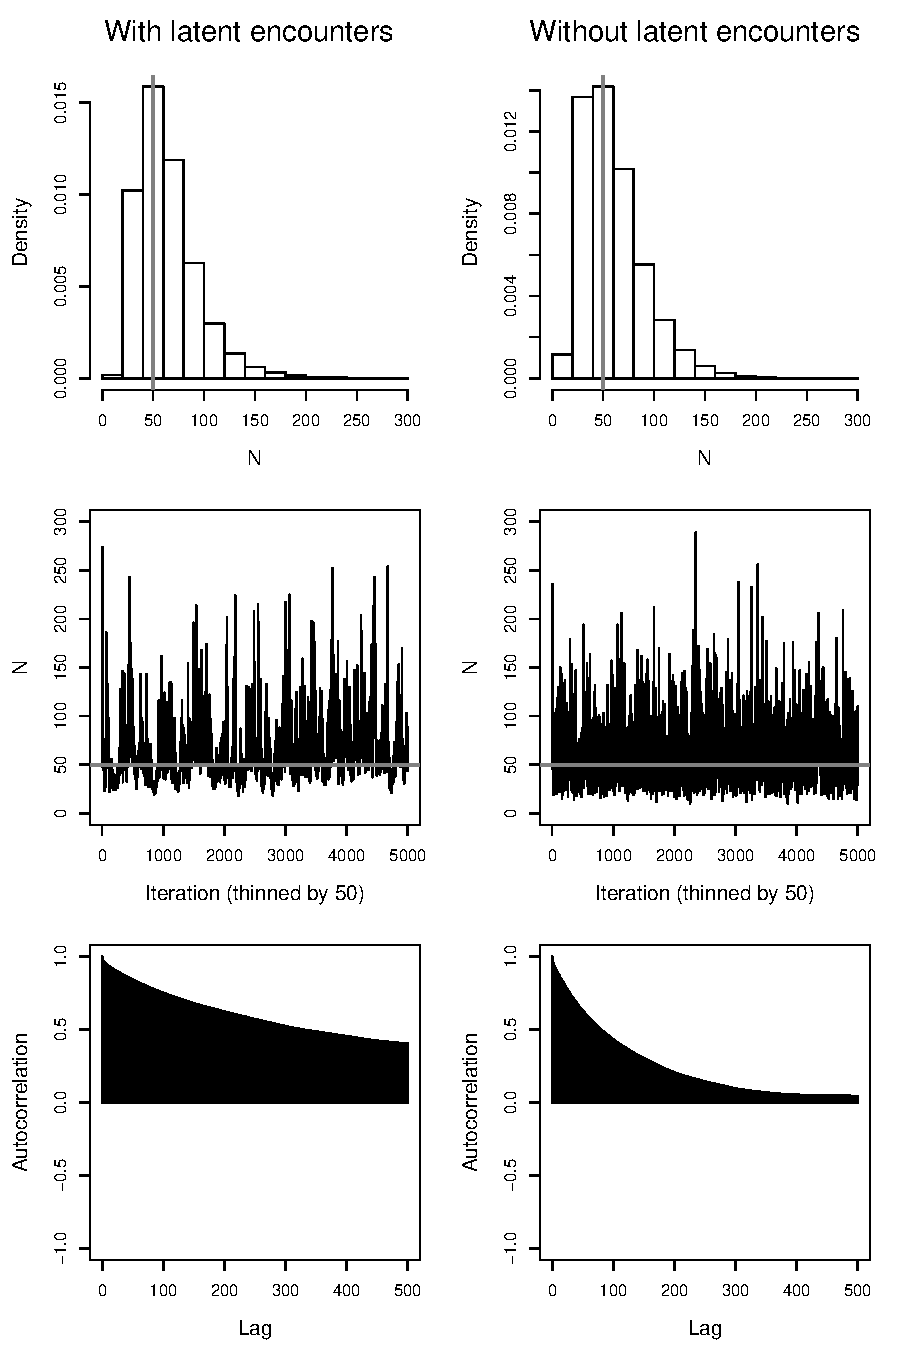
\includegraphics[width=0.8\textwidth]{Ch18-Unmarked/figs/mc1mc2}
  \caption{MCMC results for the parameter $N$ from the two algorithms
    (with and without the latent encounter histories). The first
    row contains the histograms of the posterior distributions, the second row
    contains the history (or trace) plots, the third row shows the
    autocorrelation plots.}
  \label{unmarked.fig.Nsim}
\end{figure}
% XX RS: I think I call row 2 'trace plots' in the MCMC chapter

The take-home message is that, even with simulated data,
%-- data that meet all of the model assumptions --
the precision of the posterior distributions is
low and mixing is poor. This should be expected given that we are
asking so much from so little data. In essence, we are trying to fit a
point process model while being twice removed from the actual point
(activity center) locations. These difficulties may warrant the investigation of simpler
models at the expense of the mechanistic description of the system. Another option is to
figure out ways of improving model precision -- options we discuss in
Sec.~\ref{unmarked.sec.precision}. Before doing so, we re-analyze the
Northern Parula ({\it Parula americana}) data
described in \citet{chandler_royle:2012}



%\begin{comment}

\section{The Maryland Northern Parula Study}
% XX RS: I seem to remember that we said that examples should just be the name of the study, i.e. Northern Parulas in Maryland, or something (without the word 'study')
% Also, I'd use the intro sentence you commented out.

%Here we re-analyze the northern parula ({\it Parula americana}) data
%described in \citet{chandler_royle:2012}.
The parula data are standard avian point count data, with one
exception. Typically, points are spaced by $>200$ m when studying
passerines in order to maintain statistical independence. In contrast,
the parula data were collected at
105 points located on a 50-m grid, which virtually ensures spatial
correlation since the parula song can be heard from distances $>$50 m.
%at the Patuxent Wildlife Research Center.
Each point was surveyed 3 times during June 2006, and
Fig.~\ref{fig:nopaDat} depicts the resulting spatially-correlated
counts ($n_{j.}$). A total of 226 detections were made with a maximum
count of 4 during a single survey. At 38 points, no birds were
detected. All but one of the detections were of singing males, and
this one observation was not included in the analysis.

\begin{figure}
  \centering
  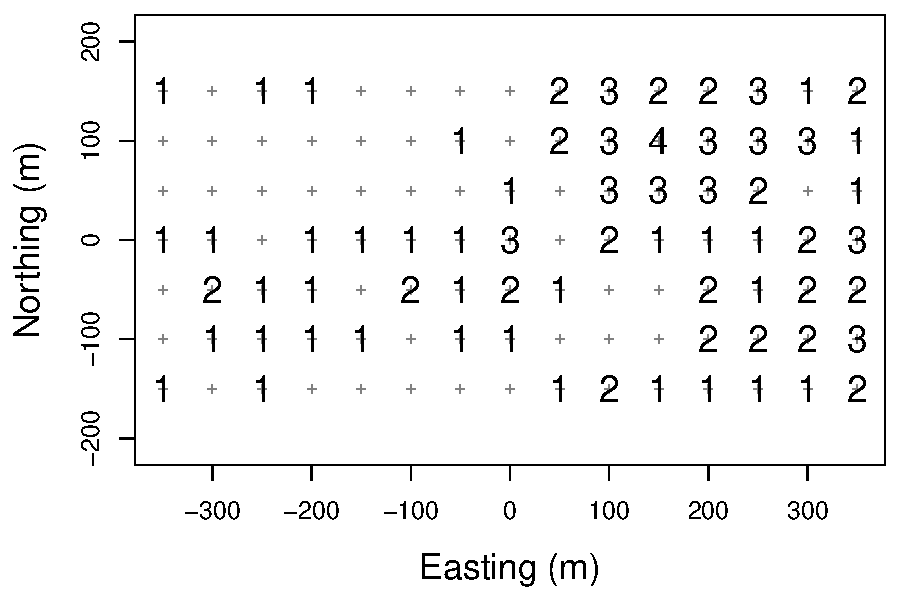
\includegraphics[width=0.8\textwidth]{Ch18-Unmarked/figs/nopaCounts}
  \caption{Spatially-correlated counts of northern parula. Gray
    crosses are the locations of the 105 point count
    stations. Superimposed are the number of detections after 3 survey occasions.}
  \label{fig:nopaDat}
\end{figure}

We fit the model using \jags~and the code from
Panel~\ref{unmarked.panel.jags2}, which does not include the latent
encounter histories. For comparative purposes, we used proper priors
rather than the improper priors used by \citet{chandler_royle:2012}, but
all other aspects of the analysis were the same, including $M=300$ and
%used both versions of the code to fit the model to the parula data.
%In our analysis, we defined the point process
a state-space created by buffering the grid of point count
locations by 250 m.
%and we set $M=200$.
%For inference, we generated three Markov chains,
%each consisting of 300000 iterations after discarding the initial 10000
%draws. %Convergence was satisfactory, as indicated by an $\hat{R}$
%statistic of $<$ 1.02 \citep{gelman_rubin:1992}.
To reduce computation time, we used the \texttt{parallel} package and
distributed 3 chains to 3 separate cores. The entire example can be
reproduced using the code on the help page for \verb+nopa+ in our
\R~package \texttt{scrbook}. The following illustrates the essential
elements:
\begin{small}
\begin{verbatim}
> library(scrbook)
> library(rjags)
> dat2 <- list(n = nopa$n, X = nopa$X, M=300, J=nrow(nopa$n), K=ncol(nopa$n),
+             xlim=c(-600, 600), ylim=c(-400, 400))
> init2 <- function() {
+    list(sigma=rnorm(1, 100), lam0=runif(1), z=rep(1, dat2$M))
+ }
> cl2 <- makeCluster(3) # Open 3 parallel R instances
> clusterExport(cl2, c("dat2", "init2", "pars1")) # send objects to 3 cores
> system.time({
+ out2 <- clusterEvalQ(cl2, { # executes the folowing command on each core
+    library(rjags)
+    jm <- jags.model("nopa2.jag", dat2, init2, n.chains=1, n.adapt=500)
+    jc <- coda.samples(jm, pars1, n.iter=2500)
+    return(as.mcmc(jc))
+ })
+ }) # 6242
> mc2 <- mcmc.list(out2) # put the 3 chains together
> plot(mc2)
> summary(mc2)
\end{verbatim}
\end{small}



\begin{comment}

\begin{table}%[t]
  \centering
  \caption{Posterior summary statistics for spatial count
    model applied to the northern parula data. Two sets of priors were
    considered. }
%  \small
  \begin{tabular}{l l rrrrrr}
    \hline
    Par          & Prior          & Mean  & SD    & Mode  & 2.5\% & 50\% & 97.5\% \\
    \hline
    $\sigma$     & $U(0, \infty)$ & 2.15  & 1.22  & 1.23  & 0.90   & 1.67  & 5.17   \\
    $\lambda_0$  & $U(0, \infty)$ & 0.28  & 0.15  & 0.21  & 0.08   & 0.26  & 0.67   \\
    $N$          & $U(0, M)$      & 40.95 & 38.07 & 4.00  & 3.00   & 31.00 & 143.00 \\
    \hline
%    $\sigma$    & $G(13, 10)$    & 1.30  & 0.26  & 1.23  & 0.90   & 1.27  & 1.91   \\
%    $\lambda_0$ & $U(0, \infty)$ & 0.30  & 0.13  & 0.24  & 0.10   & 0.28  & 0.60   \\
%    $N$         & $U(0, M)$      & 59.32 & 36.49 & 36.00 & 18.00  & 50.00 & 157.00 \\
%    $D$         & --             & 0.62  & 0.38  & 0.38  & 0.19   & 0.52  & 1.64   \\
    \hline
  \end{tabular}
  \label{unmarked.tab.nopa}
%\vspace{0.5cm}
\end{table}

\end{comment}

XXXX THE RESULTS OF THE TWO ANALYSES LOOK VERY SIMILAR AS EXPECTED XXXX
%%%%% Andy sez: Sounds good to me.


Several aspects of this analysis could be improved via model
extensions. In particular, we note that a more appropriate observation
model would recognize the fact that detection in this case is the
result of two processes. Specifically, an ideal encounter probability
model would include a process describing the location of the bird (not
just its home range center) as well as the probability of detecting
it, given its location during the survey.
% XX RS: This sounds similar to the search-encounter formulation
Essentially, the model we
would like to fit could be thought of as a latent distance sampling
model allowing for movement. As it turns out,
a very rudimentary form of distance data were collected -- birds were
determined to be either within 150 m or beyond 150 m from the
observer. In Sec.~\ref{unmarked.sec.ext}, we
propose a model to accommodate these auxiliary data.

% XX RS: You end sections a  lot by referring to the next section. Maybe look through section endings and reduce that a little, or sometimes use indirect references - '(see sec. XXX)' instead of a full sentence.



%\end{comment}


\section{Improving Precision}
\label{unmarked.sec.precision}

%\subsection{Prior information}

%We are asking a lot of a little data. Because both the activity
%centers and the encounter histories are latent variables, there is
%inherently high uncertainty in the data, even if it is ``perfect''
%data simulated from the true model. This explains the low posterior
%precision in the parula data.

\citet{chandler_royle:2012} recommended two strategies for improving
the precision of the posterior distributions obtained under the SC
model: (1) mark a subset of individuals or (2) elicit informative
priors from the published literature.
% XX RS: Might be good to say for which parameters.
The first option is the subject of the next chapter. The second option
should be readily accomplished in many studies %of unmarked populations
because extensive information on home range size has
been compiled for many species in diverse habitats %\emph{e.g.}
\citep[\emph{e.g.},][]{degraaf_yamasaki:2001}. It is
easy to embody this information as a prior distribution in Bayesian
analyses (\citet{chandler_royle:2012}, Chapt.~\ref{chapt.scr0}).

\begin{comment}
  One benefit of a Bayesian analysis is that it can accommodate prior
  information on the home range size and encounter rate parameters,
  which are readily available for many species. To illustrate, we
  analyzed the parula data using a new set of priors. Whereas in the
  first analysis, all priors were improper, customary non-informative
  priors (see Table \ref{t:nopaPosts}), in the second set we used an
  informative prior for the scale parameter $\sigma \sim
  \mbox{Gamma}(13,10)$. We arrived at this prior using the methods
  described by \citet{royle_etal:2011mee} and published information on
  the warbler's home range size and detection probability
  \citep{moldenhaer_regelski:1996,simons_etal:2009}. More details on
  this derivation are found in ??????. We briefly note here that this
  prior includes the biologically-plausible range of values from
  $\sigma$ suggested by the published literature.


  This was true when considering both sets of priors, although
  posterior precision was higher under the informative set of
  priors. Specifically, the use of prior information reduced posterior
  density at high, biologically implausible, values of $\sigma$, and
  hence decreased the posterior mass for low values of $N$
  (Fig.~\ref{fig:prior}).
\end{comment}

In some cases, it may not be possible to mark any individuals, and no
prior information may exist about encounter parameters; however, it
may be possible to collect axillary data, such as the distance
measurements recorded in the parula study.
Other sources of auxiliary data could include removal counts of
double observer counts, which are routinely collected in
wildlife studies. Extending the model to accommodate such data is
treated in the next section.




\section{Extensions of the Spatial Count Model}
\label{unmarked.sec.ext}

%Noting the relatively low precision of the posterior distributions,

%In this section, we describe model extensions for accomodating
%auxiliary data as a means of increasing posterior precision. Buy

If ancillary data such as distance measurements exist, why
%would we
bother with the SC model at all?
%at all when data such as distance measurements are available?
Isn't density estimable
using the distance data alone? Yes, in fact it is, and in many situations a
simple distance sampling model will be sufficient. However, unlike the
situation we described earlier in this chapter where we viewed spatial
correlation as a good thing, the model extension we describe now
provides a means of dealing with spatial correlation when it is
unwanted or perhaps unavoidable.
% XX RS: Next sentencce looks like a Frankenstein of several sentences. :)
In addition, extensions of this model
We suspect that the SC model could
can be used to make inferences about multiple processes in addition to
spatial and temporal variation, such as home range size and movement.
%extended to include
%this ancillary data and thereby allow for inference about three
%processes: density, home range size, and
%distance-related heterogeneity in detection probability.
%In addition
%to providing information about multiple processes of interest, it
%seems likely that the estimates would be more precise than those of
%the basic model. Also, note that this provides a mechanism for
%modeling spatial correlation in distance sampling, a topic which has
%recieved little attention \citep{hedley_etal:1999,niemi_fernandez:2010}.
%In Sec.~\ref{unmarked.sec.ext}, we
%elaborate on similar model extensions.
%In addition, extensions of this model
%can be used studying spatial and temporal variation in density as well as
%home range size and movement.

As an example, consider again the northern parula data.
%analyzed by
%\citet{chandler_royle:2012}. These point count locations were spaced
%by only 50 m, and since the song of the parula can be easily heard
%from a distance of $>100$ m, the neighboring counts exhibit
%correlation.
As it turns out, %the data collected were more than just
%the simple counts -- the
observers recorded rudimentary distance sampling data by determining
if each detected
individual was within or beyond 100 m. Although not ideal, distance
data binned into 2 intervals are sufficient for estimating the scale
parameter of a distance sampling detection function, and thus we
should be able to use that information to increase precision
% XX RS: Precision of what?
and
develop a more realistic encounter model. % in our expanded model.
Doing so requires that we consider not only the activity centers,
but also the actual locations of individuals during each survey --
much like in search-encounter models
(Chapt.~\ref{chapt.search-encounter}). %In fact, the model we are about
%to describe is essentially a hybrid SC and search-encounter
%model. First, consider another example.

By including both activity centers ({\bf s}) and actual locations
({\bf u}) in the model, abundance in any region
$\mathcal{B}$ is given by
% XX RS: Ok, but locations can change across occasions, so that is an occasion-specific regional abundance? Would be nice to be clearer about that aspect.
\begin{equation}
N(\mathcal{B}) = \sum_i I({\bf u}_i \in \mathcal{B}).
\label{unmarked.eq.B}
\end{equation}
Thus, in the context of distance sampling studies in which the
distance data are recorded in discrete intervals, the region
$\mathcal{B}$ would be the area corresponding to a particular distance
interval. The probability of detecting the individuals
$N(\mathcal{B})$ would be the average detection probability $\bar{p}$,
which is computed by integrating a distance-based detection function
over the distance interval.

In other contexts, such as when conducting removal surveys, the region
$\mathcal{B}$ could be a fixed-area plot, such as a stream
segment. Again, Eq.~\ref{unmarked.eq.B} could be used to model local
abundance ($n(\mathcal{B})$), and detection probability within the region could be
modeled conditional on $n(\mathcal{B})$. For instance, if a stream
segment is uniformly surveyed using electrofishing equipment, then a
standard non-spatial removal model could be used to estimate detection
probability $p$, conditional on the spatially-explicit model of
abundance. A reasonably general description of this model is as
follows:
% XX RS: substitute BiNormal with BVN
%% Andy sez: I noticed this too -- and made the change
\begin{gather*}
  {\bf s}_i \sim \text{Uniform}(\mathcal{S}) \\
  {\bf u}_{ik} \sim \text{BVN}({\bf s}_i, \tau) \\
  N(\mathcal{B}_{jk}) = \sum_{i=1}^M I({\bf u}_{ik} \in \mathcal{B}_{jk}) \\
  n_{jkl} \sim \text{Binomial}(N(\mathcal{B}_{jkl}), p)
\end{gather*}
%where $\mathcal{B}$ is the region associated with some distance
%interval used during data collection. For example, $\mathcal{B}_1$
%could be the region within 10 m of a survey point, or the annulus
%comprising the 10-20 m interval.
where $\tau$ is the parameter of a bivariate normal distribution (with
correlation $\rho=0$) describing the locations of individuals on occasion
$k$. The interpretation of the parameter $p$ will depend upon the
survey protocol.

\begin{comment}
  a movement parameter describing the probability that an individual
  occurs at location $\bf u$ given it's activity center. The number of
  individuals that occur in each $\mathcal{B}$ are then detected with
  probability $\bar{p}$, which is computed

  We have considered the case where distance data are collected in
  intervals or are binned after the fact, but the model could be
  easily extended to allow for continuous distance measurements.

  Another related extension applies to data collected in fixed area
  plots, such as fixed-radius point count studies, or area
  searches. In such studies, researchers often make multiple visits to
  a plot and record the number of individuals detected. In animal
  studies, a common problem is that individuals move on and off the
  plots and this, what is known as temporary emigration, makes it
  difficult to determine the effective sample size, just as in
  traditional non-spatial capture-recapture studies.
\end{comment}

When plots are far enough apart that
individuals cannot move between them, the counts will be uncorrelated
and the model can be approximated using a non-spatial $N$-mixture model
allowing for temporary emigration \citep{chandler_etal:2011}.
In the next example, we consider data in which the plots are obviously
not independent.


\section{The Maryland Dusky Salamander Study}
% XX RS: Same as for Parula title
The independence assumption of the \citet{chandler_etal:2011} model
will not always hold. A prime example is in studies of aquatic
species in stream networks. For example, consider the data depicted in
Fig.~\ref{unmarked.fig.salct}. What is this spaghetti soup, you say?
% XX RS: Nice!
These
are streams of numbers corresponding to counts of northern dusky salamanders
(\textit{Desmognathus fuscus}) in 25-m stretches on a small stream in the Chesapeake and
Ohio National Historic Park. The data were collected by E.H.C. Grant
and colleagues with the objective of understanding the spatial and
temporal dynamics of salamander populations in response to seasonal
and annual variations in stream
hydrology. In addition, movement processes, including dispersal are
studied between years (see \citet{grant_etal:2010} for more
details).
% XX RS: This sentence seems incomplete
% \citep{grant_etal:2007}

To sample the population, the stream networks are divided into 25-m
stretches % in numerous streams such
as illustrated in Fig.~\ref{unmarked.fig.salct}. In each
stretch, ``temporary'' removal sampling is used, which involves
%make 3 passes,
capturing and removing salamanders on 3 consecutive passes. The
salamanders are placed in a bucket of water for the brief 10-20 min
duration of sampling, and then they are released at the location of
capture. The entire process is repeated 3-4 times per season (May-Aug).
In a subset of streams and years, individuals
are marked, but in general it is too expensive to mark the entire
population, and the data considered here consists entirely of unmarked individuals.
% XX RS: I am curious - how do you mark a salamander? Surely not with an ear tag...

\begin{figure}
  \centering
  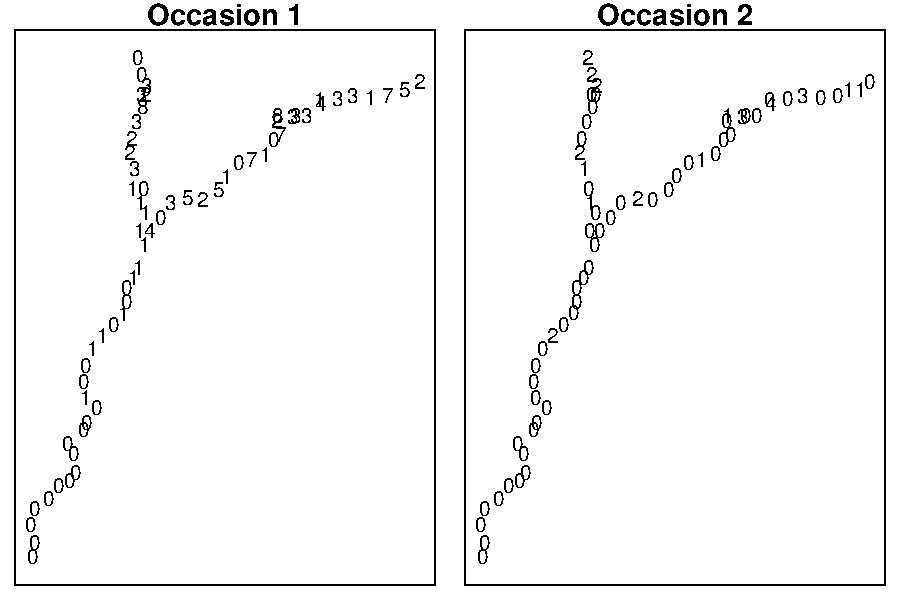
\includegraphics[width=0.8\textwidth]{Ch18-Unmarked/figs/saln27}
  \caption{Stream segment counts of northern dusky salamanders
    in the Chesapeake and Ohio National Historic Park,
    VA/MD. Each number is the count associated with a 25-m stretch in which 3 removal passes
    were made on 3 occasions each summer (only 2 occasions are shown
    here). Notice the consistency of the spatial correlation between
    occasions and the temporal decline in the counts.}
  \label{unmarked.fig.salct}
\end{figure}


The sampling protocol may be
thought of as a ``robust design'' \citep{pollock:1982}, with
``occasions'' (typically 1 day) being the primary period, and
secondary samples being the removal passes within the primary
periods. An obvious feature of these data is that the neighboring
counts are spatially correlated. In this case, we have reason to
believe that this correlation is the result of habitat preferences,
with individuals actively selecting habitat in the upper reaches of
the streams. This could be modeled as a function of a covariate
describing the distance from the mouth of the stream. Another obvious
feature of this data is that the pattern of spatial correlation
remains consistent between occasions, but the overall counts decline
markedly over the course of the season.
These phenomena can be explained by the fact that the salamanders have
relatively small home ranges, and this results in the consistent pattern of
correlation  among occasions. Furthermore, as the season progresses, the
streams dry out, and many individuals move underground.

Given the importance of movement within home ranges, which determines
the correlation among occasions, and movement underground, which
results in a decreasing number of individuals being available for
sampling, it would be helpful to have a model that describes both
processes and allows for evaluation of hypotheses regarding the
effects of environmental variables. For example, one might ask how
stream flow is related to the probability that an individual remains
active.
% XX RS: ', i.e. above ground.' ?
A model describing this process could be used to predict
activity levels under future conditions. Although we do not
investigate covariate effects in this section, we do present a general
model allowing for movement among occasions, and for decreasing
availability over the season.

This expanded model is founded on the one described in the previous
section, but it also includes a removal model for the observation
process, and it includes a basic ``open'' population model to allow
for a decline in abundance over time
(Chapt.~\ref{chapt.open}). Actually, the population is not thought to
actually decline substantially during the season, but rather, the
number of individuals \textit{available} for detection declines
because many individuals move underground as the streams dry. Each of
these components is included in the \bugs~description of the
model presented in Panel~\ref{unmarked.panel.sal}.


\begin{panel}[ht]
\centering
\rule[0.05in]{\textwidth}{.03in}
\begin{small}
\begin{verbatim}
model {
phi ~ dbeta(1,1)      # "availability" parameter
tau ~ dunif(0, 1000)  # "movement parameter" of Gaussian kernel model
p ~ dbeta(1,1)        # detection prob
psi ~ dbeta(1,1)      # data augmentation parameter
for(i in 1:M) {
  z[i,1] ~ dbern(psi)        # is the guy real?
  z[i,2] ~ dbern(z[i,1]*phi) # and still alive?
  z[i,3] ~ dbern(z[i,2]*phi) # still kicking
  s[i] ~ dcat(PrSeg[]) # location (stream segment) of activity center
  for(g in 1:G) {
    PrU[i,g] <- exp(-distmat[s[i],g]^2/(2*tau^2)) # Pr(u | s)
    }
  for(k in 1:K) {
    u[i,k] ~ dcat(PrU[i,]) # location of guy i at time k
    for(g in 1:G) {
      y[i,g,k] <- (u[i,k] == g)*z[i,k] # was guy at u==g?
      }
    }
  }
for(j in 1:J) {
  for(k in 1:K) {
    N[j,k] <- sum(y[,seg[j],k]) # Number of individuals in seg j at time k
    # removal model:
    n[j,1,k] ~ dbin(p, N[j,k])
    N2[j,k] <- N[j,k] - n[j,1,k]
    n[j,2,k] ~ dbin(p, N2[j,k])
    N3[j,k] <- N2[j,k] - n[j,2,k]
    n[j,3,k] ~ dbin(p, N3[j,k])
    }
  }
Ntot[1] <- sum(z[,1]) # Abundance, occasion 1
Ntot[2] <- sum(z[,2]) # Abundance, occasion 2
Ntot[3] <- sum(z[,3]) # Abundance, occasion 3
}
\end{verbatim}
\end{small}
\rule[0.05in]{\textwidth}{.03in}
\caption{\bugs~description of model for the data shown in
  Fig.~\ref{unmarked.fig.salct}. The model allows for
  spatially-explicit temporary emigration, and for a decrease in
  abundance as individuals move underground throughout the course of
  the season.}
\label{unmarked.panel.sal}
\end{panel}

We fit this model to the data and obtained the posterior distributions
summarized in Table~\ref{unmarked.tab.dusky}. The results indicate that
the population size available for detection did decrease
rapidly during the season, the rate of which is determined by the
$\phi$ parameter. Modeling this parameter as a function of water flow
or volume would allow one to predict salamander activity under future
environmental conditions.
Another result of the analysis is that the movement parameter, $\tau$,
was relatively low, indicating that adult salamanders rarely move more
than 100 m
% XX RS: What's that in 'stream segments', since you have discrete movements across segments?
from their home range center during a season. This explains
why the distribution of individuals within the stream remains
relatively constant over time. Including this parameter in the model
also provides a general mechanism for modeling temporal correlation in
count data.
%peterson_etal:2013
% XX RS: One thing I wonder about and that might be worth mentioning: these movement models with u|s, they introduce another boatload of latentn variables. How does this model then do better?
% Also - this is a neat model but it does kind of move away from the original SC, no? It's a count model but it looks quite different to me; we have detection that's not spatially structured. I might not have read this section carefully enough, but it might be worth to point out the analogies.

\begin{table}
  \centering
  \caption{Posterior summarizes from removal model of salamander
    counts allowing for movement and decreasing population size over
    the course of a breeding season.}
  \begin{tabular}{lrrrrr}
    \hline
    Parameter & Mean    & SD     & 2.5\%   & 50\%    & 97.5\%  \\
    \hline
    $N_1$     & 178.393 & 16.346 & 151.000 & 177.000 & 214.000 \\
    $N_2$     & 62.322  & 6.884  & 51.000  & 62.000  & 77.000  \\
    $N_3$     & 21.202  & 3.695  & 15.000  & 21.000  & 29.000  \\
    $\phi$    & 0.348   & 0.038  & 0.275   & 0.348   & 0.425   \\
    $\tau$    & 27.427  & 3.200  & 21.293  & 27.173  & 33.706  \\
    $p$       & 0.396   & 0.053  & 0.294   & 0.394   & 0.502   \\
    \hline
  \end{tabular}
  \label{unmarked.tab.dusky}
\end{table}


\begin{comment}
  \subsection{Similarity to other data augmentation schemes}

  By including the $w$ variables in the model, we have made use of the
  data augmentation technique introduced by \citet{royle_etal:2007}
  and developed by \citep{royle:2009} and
  \citep{royle_dorazio:2010}. However, including the latent encounter
  histories in the model can also be viewed as another form of data
  augmentation, which was in fact, first proposed as a general model
  of spatial dependence in count data \citep{wolpert_ickstadt:1998}.

  The model of \citet{wolpert_ickstadt:1998} is slighly different than
  the SC model in that they defined $\{{\bf s}_1, \ldots, {\bf s}_N\}$
  not as a realization from a spatial point process, but rather as
  locations of a dense array of points, typically a fine grid covering
  the $J$ survey locations. The purpose of this grid is to introduce
  random spatial noise into the system, which is then smoothed using
  what, in our case, is the encounter model. In their case, the
  encounter model is simply a smoothing kernel that determines the
  spatial covariance structure -- if $\sigma$ is high relative to the
  ``trap'' spacing, the counts will be highly correlated, and vice
  versa. Similar ideas have been used to model spatial dependence in
  temperature data \citep{higdon:1998}. In the SC model, $\sigma$ and
  the encounter model also determine the spatial correlation, but it
  has an explicit connection to correlation as information about the
  number and location of the activity centers.

  In addition to the fact that they fixed the locations of the $\bf
  s$'s, their model also differs from the SC model in that they also
  fix $N$, it being chosen to create a suitably fine grid for
  generating the white noise.





  \subsection{Linear Designs}

  Survey points are not always located on a grid with even
  spacing---in fact, it is rare to see a perfect 10$\times$10 grid of
  points in any study because of habitat patchiness or rugged terrain
  or what have you. Instead, points are often distributed haphazardly
  or using some form of probability sampling. Such designs can still
  produce data amenable to the models we consider in this chapter if
  individuals can be encountered at multiple points, and none of the
  considerations discussed above need to be modified. But what about
  linear designs?

  In bird studies, point counts are often placed on linear
  transects. For example, the Breeding Bird Survey involves surveying
  50 points spaced by 0.5 miles. The mountain-top bird survey in the
  White Mountain National Forest involves surveying 42 transects, each
  with 20? points spaced by 250-m \citep{king_etal:2008}. For many
  species, the 0.5 mile spacing of the BBS will ensure that
  individuals are not detected at multiple points. However, in the
  mountain-top survey, it's easy to imagine that a Bicknell's Thrush
  (\emph{Catharus bicknelli}) could easily be heard from adjacent
  points. So can we apply our model to obtain density estimates with
  such simple counts?




  \subsection{Spatial point process models}


  Our model has some direct linkages to existing point process
  models. We note that the observation intensity function (i.e.,
  corresponding to the observation locations) is a compound Gaussian
  kernel similar to that of the Thomas process
  \citep[pp. 61-62]{thomas:1949, moller_waagepetersen:2004}.  Also,
  the Poisson-Gamma Convolution models \citep{wolpert_ickstadt:1998}
  are structurally similar (see also \cite{higdon:1998} and
  \cite{best_etal:2000}).  In particular, our model is such a model
  but with a {\it constant} basal encounter rate $\lambda_{0}$ and
  {\it unknown} number and location of ``support points'', which in
  our case are the animal activity centers, $\bf{s_i}$.  We can thus
  regard our model as a model for {\it estimating} the location and
  local density of support points in such models, which we believe
  could be useful in the application of convolution models.
  \citet{best_etal:2000} devise an MCMC algorithm for the
  Poisson-Gamma model based on data augmentation, which is similar to
  the component of our algorithm for updating the $z$ variables in the
  conditional-on-$z$ formulation of the model.  We emphasize that our
  model is distinct from these Poisson-Gamma models in that the number
  {\it and} location of such support points are estimated.


  If individuals were perfectly observable then the resulting point
  process of locations is clearly a standard Poisson or Binomial
  (fixed $N$) cluster process or Neyman-Scott process.  If detection
  is uniform over space but imperfect, then the basic process is
  unaffected by this random thinning.  Our model can therefore be
  viewed formally as a Poisson (or Binomial) cluster process model but
  one in which the thinning is non-uniform, governed by the encounter
  model which dictates that thinning rate increases with distance from
  the observation points. In addition, our inference objective is,
  essentially, to estimate the number of parents in the underlying
  Poisson cluster process, where the observations are biased by an
  incomplete sampling apparatus (points in space).


  As a model of a thinned point process, our model has much in common
  with classical distance sampling models \citep{buckland_etal:2001}.
  The main distinction is that our data structure does {\it not}
  include observed distances, although the underlying observation
  model is fundamentally the same as in distance sampling if there is
  only a single replicate sample and $\bf{s}_i$ is defined as an
  individual's location at an instant in time. For replicate samples,
  our model preserves (latent) individuality across samples and traps
  which is not a feature of distance sampling. We note that error in
  measurement of distance is not a relevant consideration in our
  model, and we explicitly do not require the standard distance
  sampling assumption that the probability of detection is 1 if an
  individual occurs at the survey point. More importantly, distance
  sampling models cannot be applied to data from many of the sampling
  designs for which our model is relevant. For example, many rare and
  endangered species can only be effectively surveyed using methods
  such as hair snares and camera traps that do not produce distance
  data \citep{oconnell_etal:2010}.

\end{comment}



%\section{Design issues}



\section{Summary and Outlook}

Unlike traditional models of count data used in ecology, the SC model
is parameterized in terms of \textit{individuals} -- individuals that just so
happen not to be directly observed. The reason for accommodating this
latent structure is that it provides a more mechanistic description
of ecological systems. For example, the model allows us to attach a
mechanism -- movement -- to the widely observed phenomenon of spatial
correlation in count data. In addition, by parameterizing the model in
terms of individuals, it makes it possible to incorporate data from
both marked and unmarked individuals, as will be described in the next
chapter. This ability to combine different
types of data should make it possible to
design effective monitoring programs when resources are too limited to
conduct spatially extensive capture-recapture
studies, as has been done
with non-spatial models \citep{conroy_etal:2008}.
% XX RS: Which one has been done with non-spatial models - replace CR with MR, or conduct spatially extensive CR studies?

The SC model is a conceptually simple extension of standard SCR
models, but in terms of computational requirements and latent
structure, it is perhaps at the extreme end of what is possible to do
with count data. As is always true, the harder we try to mirror
reality with our models, the harder it becomes to estimate the
parameters of the system. In this chapter, we tried to emphasize that
as conceptually appealing as the SC model may be, it is unlikely to
produce satisfying results in the absence of additional
information. However, additional information such as home range size
estimates will often be available
for many species, and if not, we have provided an alternative method of
accommodating additional data in the form of distance measurements or
removal counts. This can greatly increase precision in studies
designed to make spatially-explicit inferences about population
processes.

\begin{comment}
  In our view, the real benefits of the SC model stem from its ability
  to be extended in these ways and others, which, given the
  proliferation and abundance of data on unmarked individuals, will
  hopefully allow for more mechanistic studies of animal
  populations. However, we emphasize that data on \textit{marked}
  individuals will always be more informative than data on unmarked
  individuals, and thus it would be a shame if people viewed the
  existence of these models -- and other models for unmarked
  populations -- as a reason for abandoning capture-recapture studies!
\end{comment}


\begin{comment}

  At the other end of the spectrum is perhaps a simple Poisson
  regression. We sum up the counts at each trap and fit a model using
  a function like \verb+glm+. But what would be estimating?

  Concerns about ``statistical independence'' have prompted ecologists
  to design count-based studies such that observed random variables
  can be regarded as {\it i.i.d.} outcomes
  \citep{hurlbert:1984}. Interestingly, this often proves impossible
  in practice, and elaborate methods have been devised to model
  spatial dependence as a nuisance parameter. Our paper presents a
  modeling framework that directly confronts this view by
  demonstrating that spatial correlation carries information about the
  locations of individuals, which can be used to estimate density even
  when individuals are unmarked and distance-related heterogeneity
  exists in encounter probability.

  The SC model closely resembles another large
  class of spatial models, known as convolution models
  \citep{wolpert_ickstadt:1998,higdon:1998}. These
  models have been used for a variety of purposes such as describing oceanic
  surface temperatures and correlation in tree locations within managed
  forests. The SC model offers an improvement in
  some respects over existing convolution models because it does not
  require arbitrary decisions about the location and number of ``support
  points''. %We will clarify this later in the chapter, and briefly
  % mention how this model can be used outside of SCR contexts for general
  % purpose spatial modeling of correlated count data.

  In this paper, we confronted one of the most difficult challenges
  faced in wildlife sampling --- estimation of density in the absence
  of data to distinguish among individuals. To do so, we developed a
  novel class of spatially-explicit models that applies to spatially
  organized counts, where the count locations or devices are located
  sufficiently close together so that individuals are exposed to
  encounter at multiple devices. This design yields correlation in the
  observed counts, and this correlation proves to be informative about
  encounter probability parameters and hence density.  We note that
  sample locations in count-based studies are typically {\it not}
  organized close together in space because conventional wisdom and
  standard practice dictate that independence of sample units is
  necessary \citep{hurlbert:1984}. Our model suggests that in some
  cases it might be advantageous to deviate from the conventional
  wisdom if one is interested in direct inference about density. Of
  course, this is also known in the application of standard spatial
  capture-recapture models \citep{borchers_efford:2008} where
  individual identity is preserved across trap encounters, but it is
  seldom, if ever, considered in the design of more traditional count
  surveys.

  Our model has broad relevance to an incredible number of animal
  sampling problems. Our motivating problem involved bird point counts
  where individual identity is typically not available. The model also
  applies to other standard methods used to sample unmarked
  populations, such as camera traps or even methods that yield sign
  ({\it e.g.} scat, track) counts indexed by space. However, results
  of our simulation study reveal some important limitations of the
  basic estimator applied to situations in which none of the
  individuals can be uniquely identified. In particular, posterior
  distributions are highly skewed in typical small to moderate sample
  size situations and posterior precision is low.

\end{comment}



